\chapter{Implementation and Results}

\section{Introduction}

This chapter presents the implementation details of JKart, including service implementation, frontend development, deployment procedures, and results with screenshots demonstrating the working application.

\section{Backend Implementation}

\subsection{Service Registry Implementation}

The Service Registry uses Spring Cloud Netflix Eureka:

\begin{verbatim}
@EnableEurekaServer
@SpringBootApplication
public class ServiceRegistryApplication {
    public static void main(String[] args) {
        SpringApplication.run(ServiceRegistryApplication.class, args);
    }
}
\end{verbatim}

Configuration in \texttt{application.yml}:
\begin{itemize}
    \item Server port: 8761
    \item \texttt{register-with-eureka: false} (server doesn't register itself)
    \item \texttt{fetch-registry: false}
    \item Dashboard accessible at \texttt{http://localhost:8761}
\end{itemize}

\begin{figure}[h!]
\centering
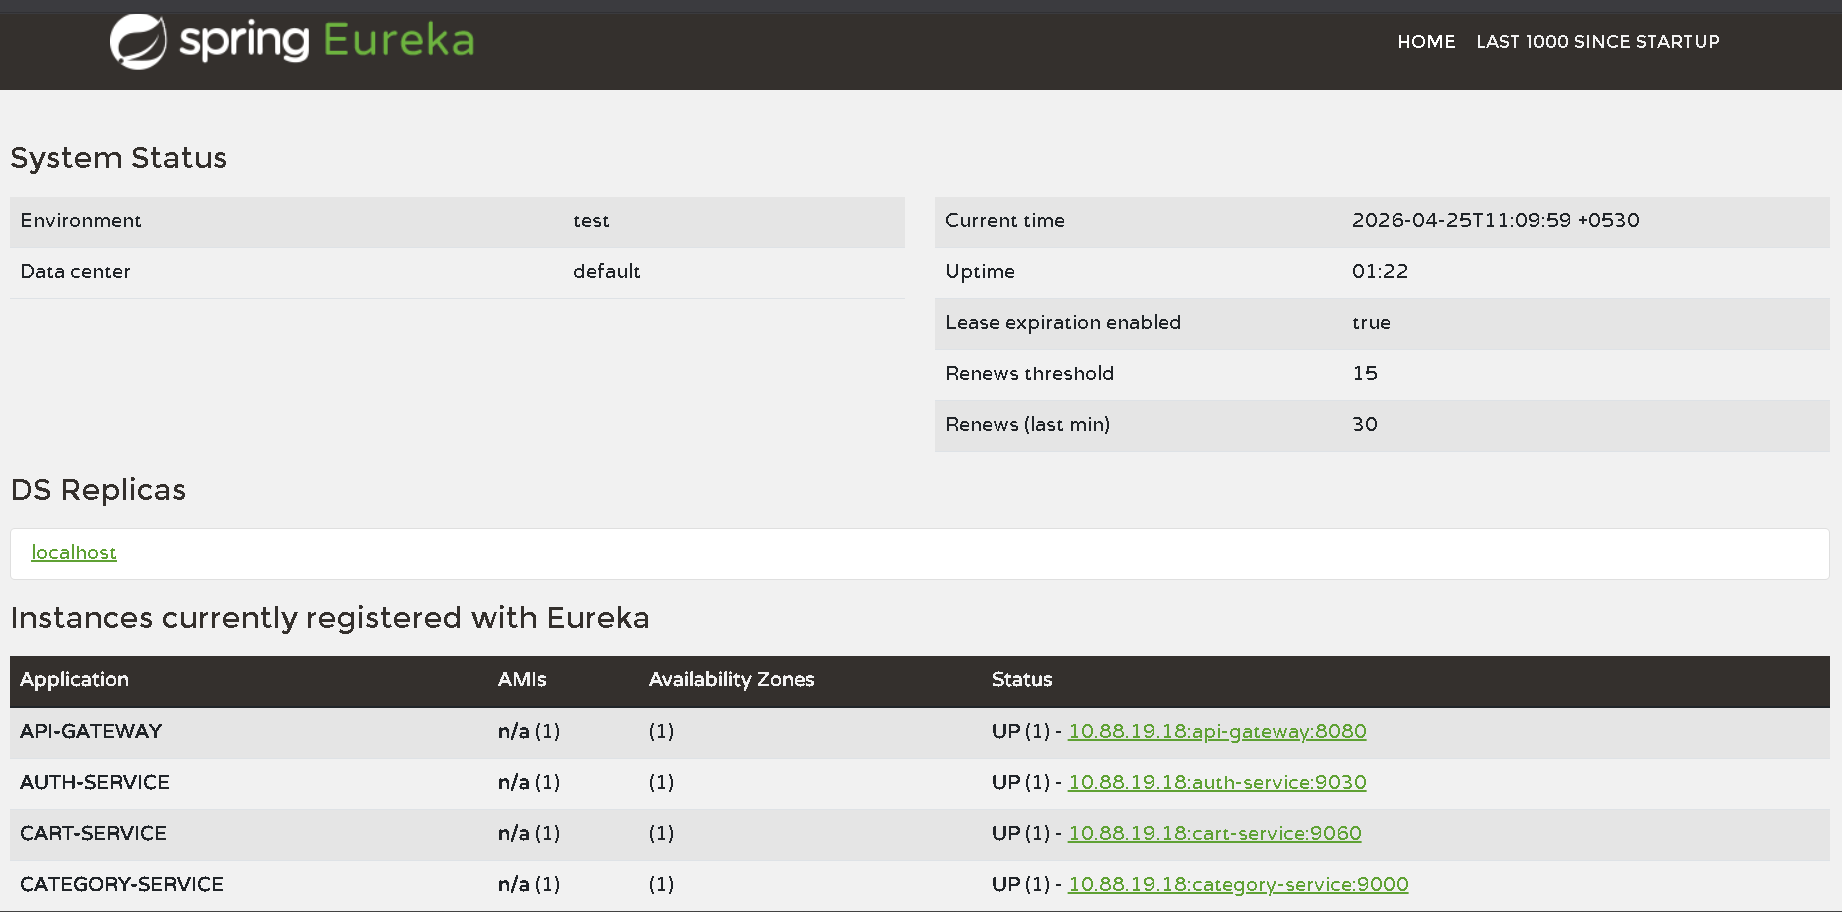
\includegraphics[width=0.75\textwidth]{eureka_server.png}
\caption{Eureka Service Registry Dashboard showing registered services}
\label{fig:eureka}
\end{figure}

\subsection{API Gateway Implementation}

Spring Cloud Gateway configured with reactive routing:

\begin{verbatim}
spring:
  cloud:
    gateway:
      routes:
        - id: auth-service
          uri: lb://AUTH-SERVICE
          predicates:
            - Path=/api/auth/**
        - id: product-service
          uri: lb://PRODUCT-SERVICE
          predicates:
            - Path=/api/product/**
\end{verbatim}

Key features:
\begin{itemize}
    \item Load-balanced routing using Eureka service names (\texttt{lb://})
    \item CORS configuration allowing frontend origin (\texttt{http://localhost:5173})
    \item Global filters for request logging
    \item Runs on port 8080
\end{itemize}

\subsection{Auth Service Implementation}

Core authentication logic with JWT and OTP:

\textbf{User Registration:}
\begin{enumerate}
    \item Receive signup request with email, password, name
    \item Validate email format and check duplicates
    \item Hash password with BCrypt (\texttt{BCryptPasswordEncoder})
    \item Generate 6-digit random OTP
    \item Set \texttt{enabled = false} and \texttt{otpExpiry = now + 10 minutes}
    \item Save user to MongoDB \texttt{js\_auth\_service} database
    \item Call Notification Service via Feign to send OTP email
    \item Return success response
\end{enumerate}

\textbf{JWT Token Generation:}
\begin{verbatim}
public String generateToken(User user) {
    return Jwts.builder()
        .setSubject(user.getEmail())
        .claim("userId", user.getId())
        .claim("roles", user.getRoles())
        .setIssuedAt(new Date())
        .setExpiration(new Date(System.currentTimeMillis() + 86400000))
        .signWith(SignatureAlgorithm.HS256, secretKey)
        .compact();
}
\end{verbatim}

\textbf{Token Validation:}
\begin{itemize}
    \item Extract Bearer token from Authorization header
    \item Parse JWT and validate signature
    \item Check expiration date
    \item Return user details if valid
    \item Other services call \texttt{/auth/isValidToken} endpoint
\end{itemize}

\subsection{Product Service Implementation}

Product catalog with search and filtering:

\textbf{Search Implementation:}
\begin{verbatim}
@GET("/api/product-service/product/search")
List<Product> searchProducts(@Param("query") String query);

// MongoDB query
public List<Product> searchProducts(String query) {
    Pattern pattern = Pattern.compile(query, Pattern.CASE_INSENSITIVE);
    return productRepository.findByNameRegexOrDescriptionRegex(pattern);
}
\end{verbatim}

Features:
\begin{itemize}
    \item Case-insensitive search across name, description, category
    \item Pagination with \texttt{Pageable} (default 20 items per page)
    \item Category filtering via \texttt{categoryId} parameter
    \item Price range filtering with \texttt{minPrice} and \texttt{maxPrice}
    \item Admin endpoints secured with \texttt{@PreAuthorize("hasAuthority('ROLE\_ADMIN')")}
\end{itemize}

\subsection{Cart Service Implementation}

Shopping cart with validation:

\textbf{Add to Cart Flow:}
\begin{enumerate}
    \item Receive cart item request (userId, productId, quantity)
    \item Call User Service via Feign: validate user exists
    \item Call Product Service via Feign: validate product and get price
    \item Check if item already in cart
    \item If exists: update quantity
    \item If new: add item with product details
    \item Calculate total price
    \item Save to \texttt{js\_cart\_service} database
\end{enumerate}

\textbf{Feign Client Example:}
\begin{verbatim}
@FeignClient(name = "PRODUCT-SERVICE")
public interface ProductClient {
    @GetMapping("/api/product-service/product/get/byId/{id}")
    ProductDTO getProductById(@PathVariable String id);
}
\end{verbatim}

\subsection{Order Service Implementation}

Order placement with mock payment:

\textbf{Create Order Flow:}
\begin{enumerate}
    \item Receive order request (userId, address)
    \item Call Cart Service via Feign: fetch user's cart items
    \item Validate cart is not empty
    \item Calculate total amount from cart items
    \item Create order record with status = "PENDING"
    \item Simulate payment processing (mock success)
    \item Update order status to "SUCCESS"
    \item Call Notification Service: send confirmation email
    \item Call Cart Service: clear user's cart
    \item Return order confirmation with order ID
\end{enumerate}

\textbf{Note:} Payment is mock/demo only - no real payment gateway (Stripe/PayPal) integrated.

\subsection{Notification Service Implementation}

Email sending via JavaMail/SMTP:

\begin{verbatim}
spring:
  mail:
    host: sandbox.smtp.mailtrap.io
    port: 2525
    username: <mailtrap-username>
    password: <mailtrap-password>
\end{verbatim}

Email templates:
\begin{itemize}
    \item \textbf{OTP Email:} Contains 6-digit verification code with expiry time
    \item \textbf{Order Confirmation:} Contains order ID, items list, total amount, delivery address
    \item Branded with JKart styling and Deep Purple theme
\end{itemize}

\section{Frontend Implementation}

\subsection{React Application Structure}

\begin{verbatim}
frontend/src/
|-- api-service/        # Axios API calls
|-- components/         # Reusable UI components
|-- contexts/           # React Context (AuthContext)
|-- pages/              # Route-based pages
|-- routes/             # React Router configuration
|-- App.jsx             # Main application component
`-- main.jsx            # Entry point
\end{verbatim}

\subsection{Authentication Flow}

\begin{enumerate}
    \item User navigates to \texttt{/auth/register}
    \item Enters email, password, first name, last name
    \item Submits form $\rightarrow$ API call to \texttt{/api/auth/signup}
    \item Redirected to \texttt{/auth/verify} to enter OTP
    \item Submits OTP $\rightarrow$ API call to \texttt{/api/auth/signup/verify}
    \item Redirected to \texttt{/auth/login}
    \item Enters credentials $\rightarrow$ receives JWT token
    \item Token stored in \texttt{localStorage}
    \item Redirected to homepage
\end{enumerate}

\textbf{AuthContext:}
\begin{verbatim}
const [user, setUser] = useState(null);
const login = (token, userData) => {
    localStorage.setItem('token', token);
    localStorage.setItem('user', JSON.stringify(userData));
    setUser(userData);
};
\end{verbatim}

\subsection{Product Browsing}

\begin{figure}[h!]
\centering
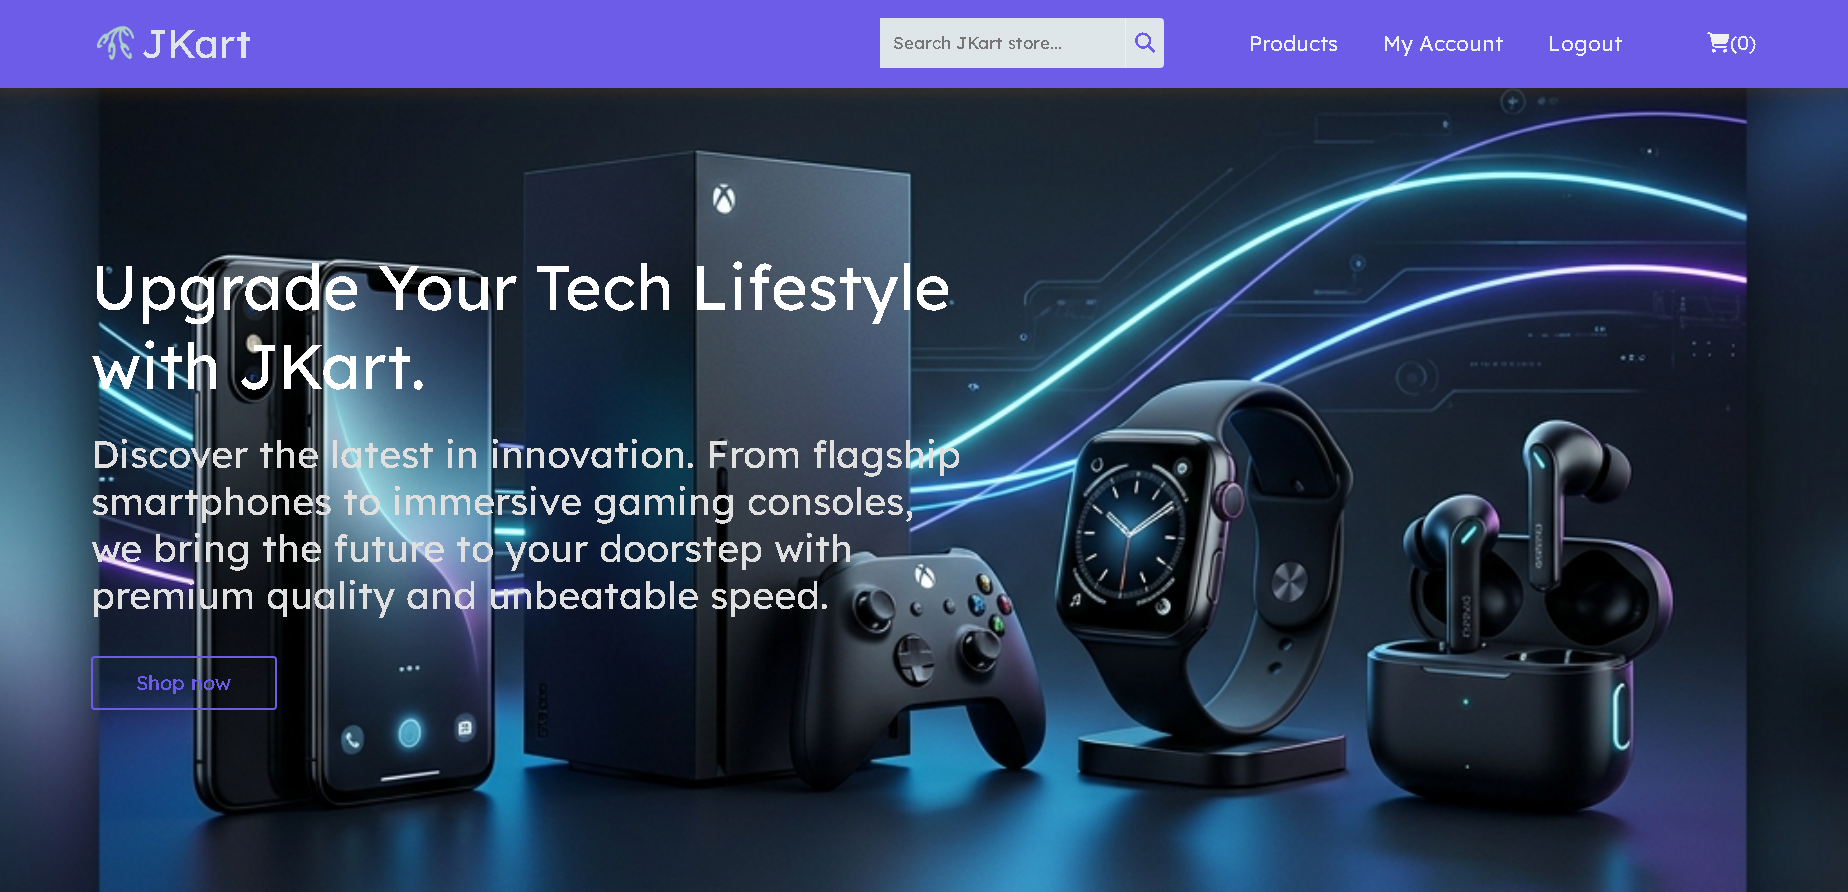
\includegraphics[width=0.85\textwidth]{home_page.png}
\caption{JKart Homepage displaying product listings with Deep Purple theme}
\label{fig:homepage}
\end{figure}

Features:
\begin{itemize}
    \item Navbar with search bar and cart icon
    \item Category sidebar for filtering
    \item Product grid with cards showing image, name, price
    \item "Add to Cart" button on each product
    \item Responsive layout for mobile devices
\end{itemize}

\begin{figure}[h!]
\centering
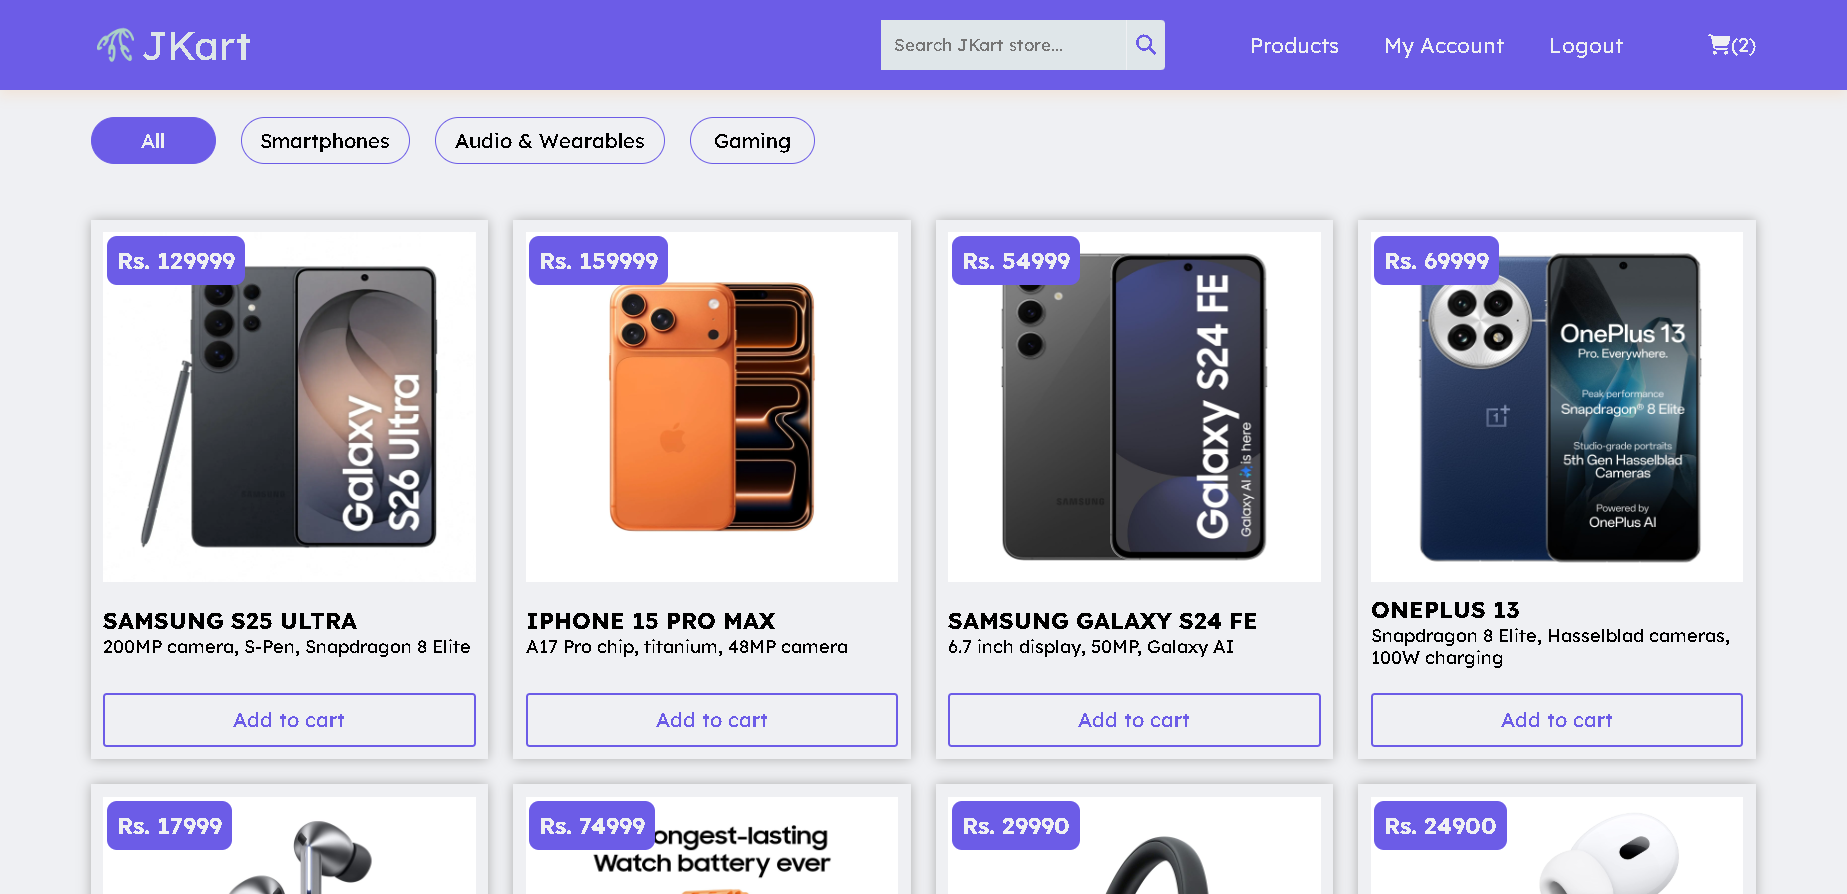
\includegraphics[width=0.85\textwidth]{products_page.png}
\caption{Products page with category filtering}
\label{fig:products}
\end{figure}

\subsection{Shopping Cart}

Cart implemented as sidebar component:

\begin{figure}[h!]
\centering
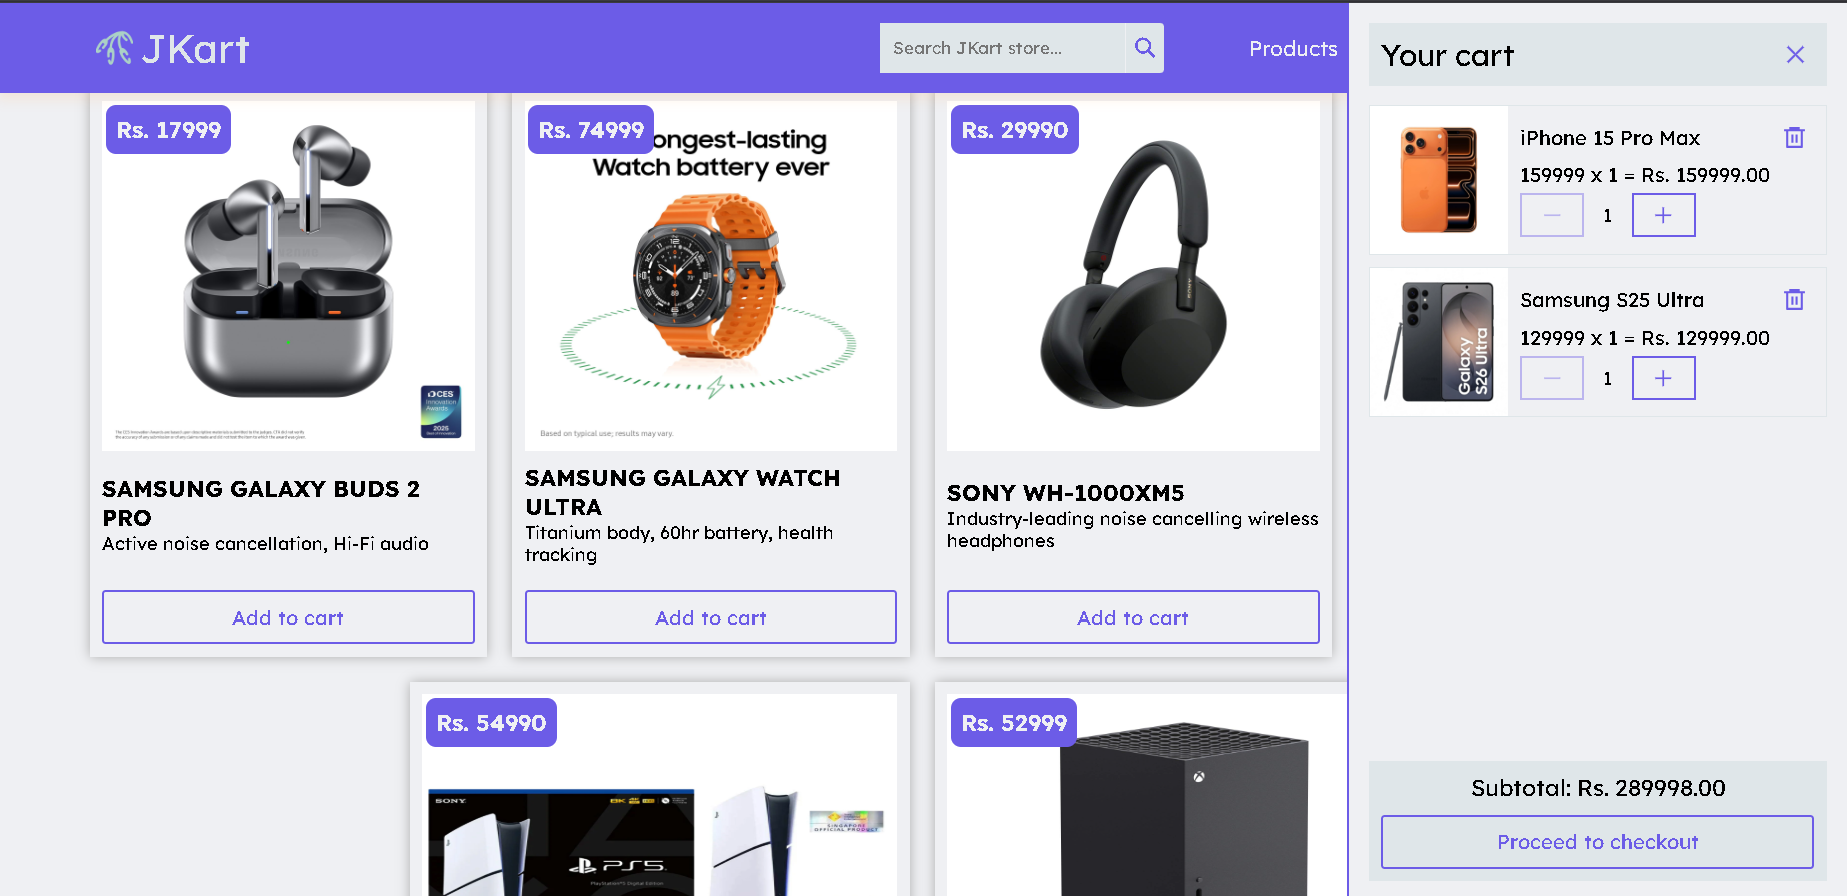
\includegraphics[width=0.75\textwidth]{cart_page.png}
\caption{Shopping cart sidebar with items and total}
\label{fig:cart}
\end{figure}

Features:
\begin{itemize}
    \item Slide-in sidebar from right
    \item List of cart items with quantity controls
    \item Update quantity or remove item
    \item Display total price
    \item "Checkout" button to proceed to order
\end{itemize}

\subsection{Checkout and Order Placement}

\begin{figure}[h!]
\centering
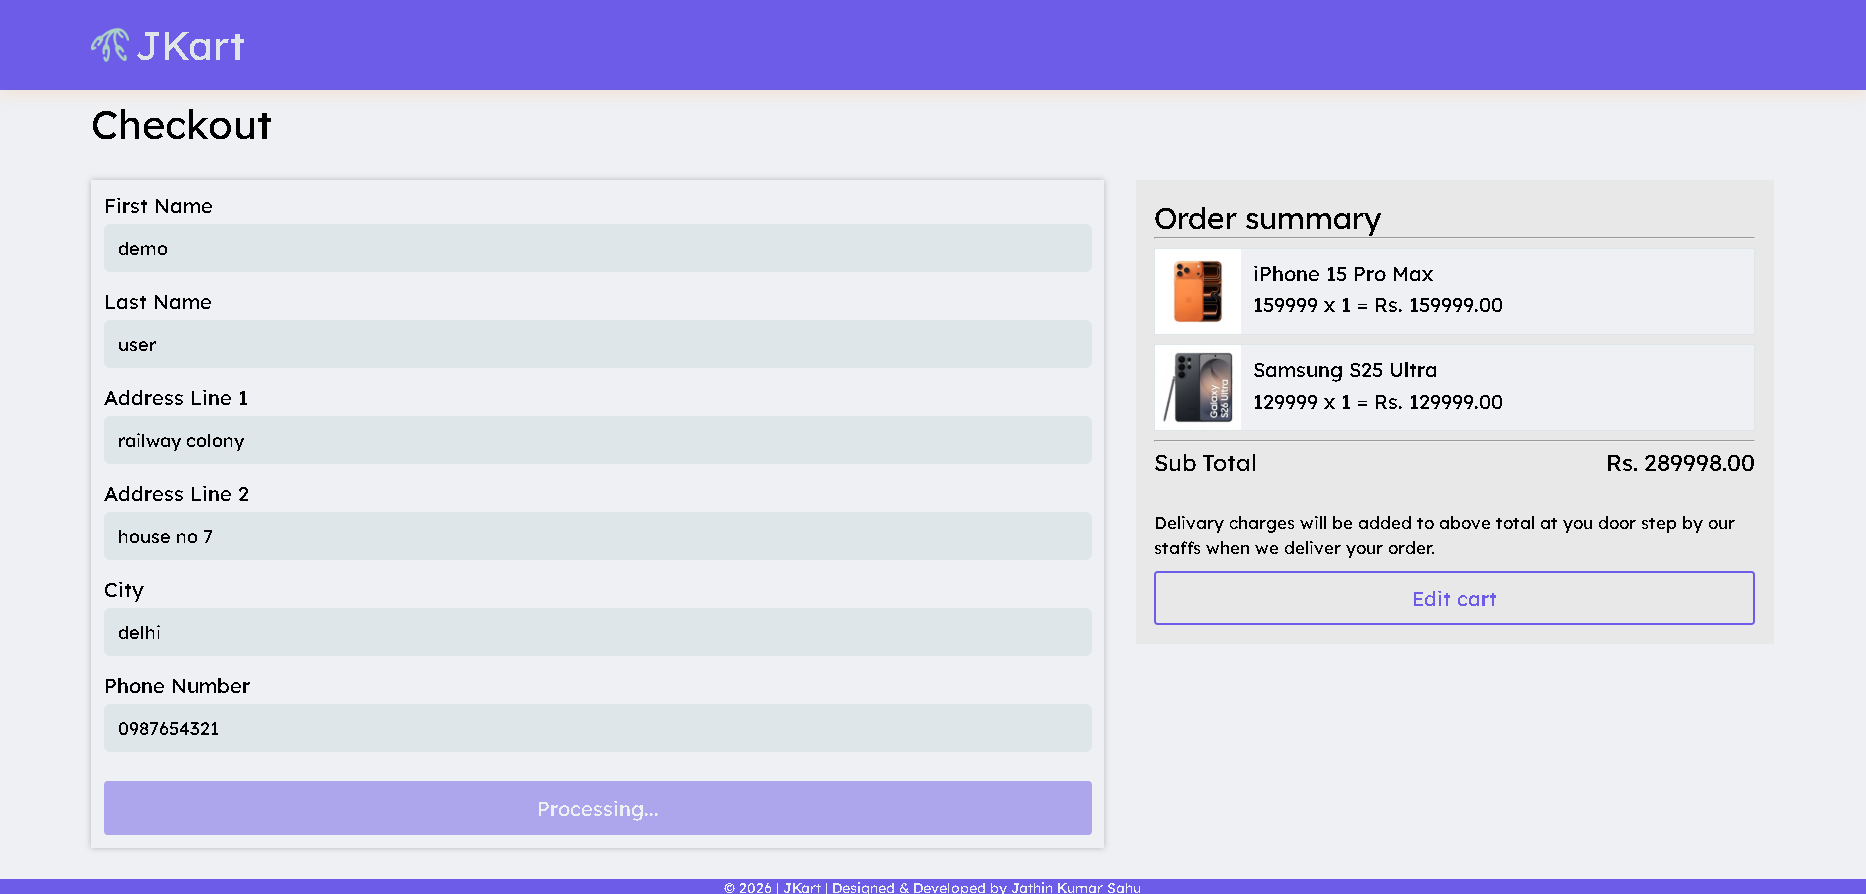
\includegraphics[width=0.85\textwidth]{checkout_page.png}
\caption{Checkout page with delivery address form}
\label{fig:checkout}
\end{figure}

Checkout flow:
\begin{enumerate}
    \item User clicks "Checkout" from cart
    \item Navigates to \texttt{/checkout} page
    \item Enters delivery address (name, phone, street, city, state, pincode)
    \item Reviews order summary (items, total)
    \item Clicks "Place Order"
    \item API call to \texttt{/api/order/create}
    \item Receives order confirmation
\end{enumerate}

\begin{figure}[h!]
\centering
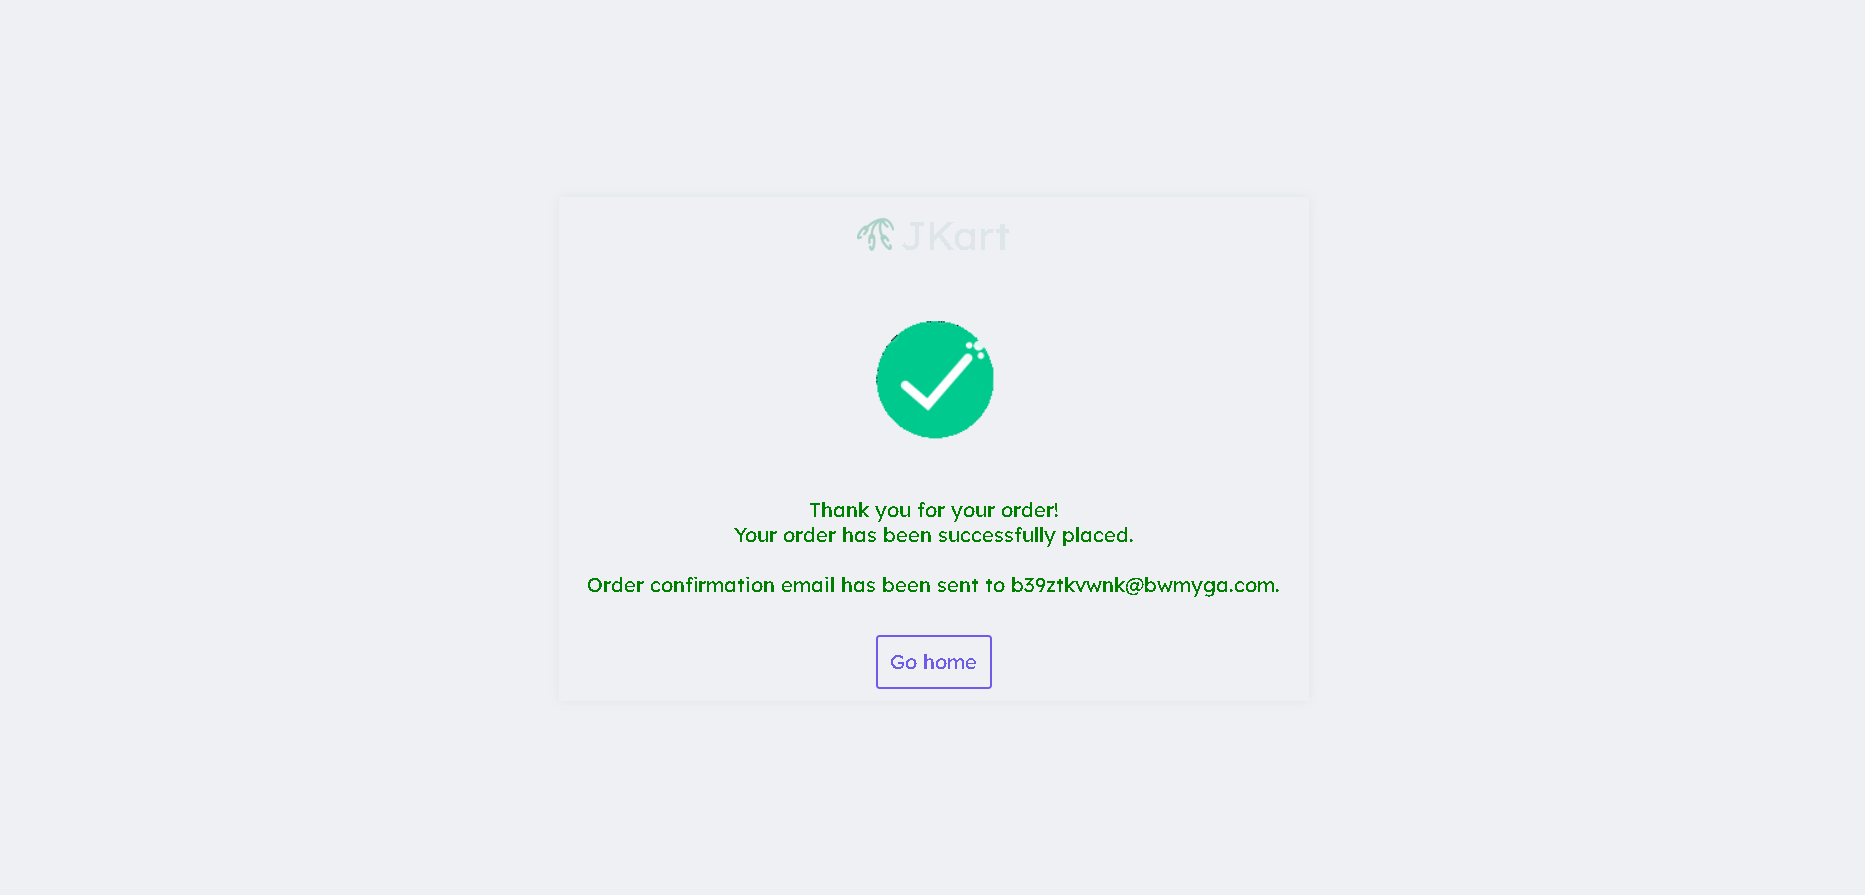
\includegraphics[width=0.85\textwidth]{order_confirmation.png}
\caption{Order confirmation page with order ID}
\label{fig:orderconfirm}
\end{figure}

\subsection{Order History}

\begin{figure}[h!]
\centering
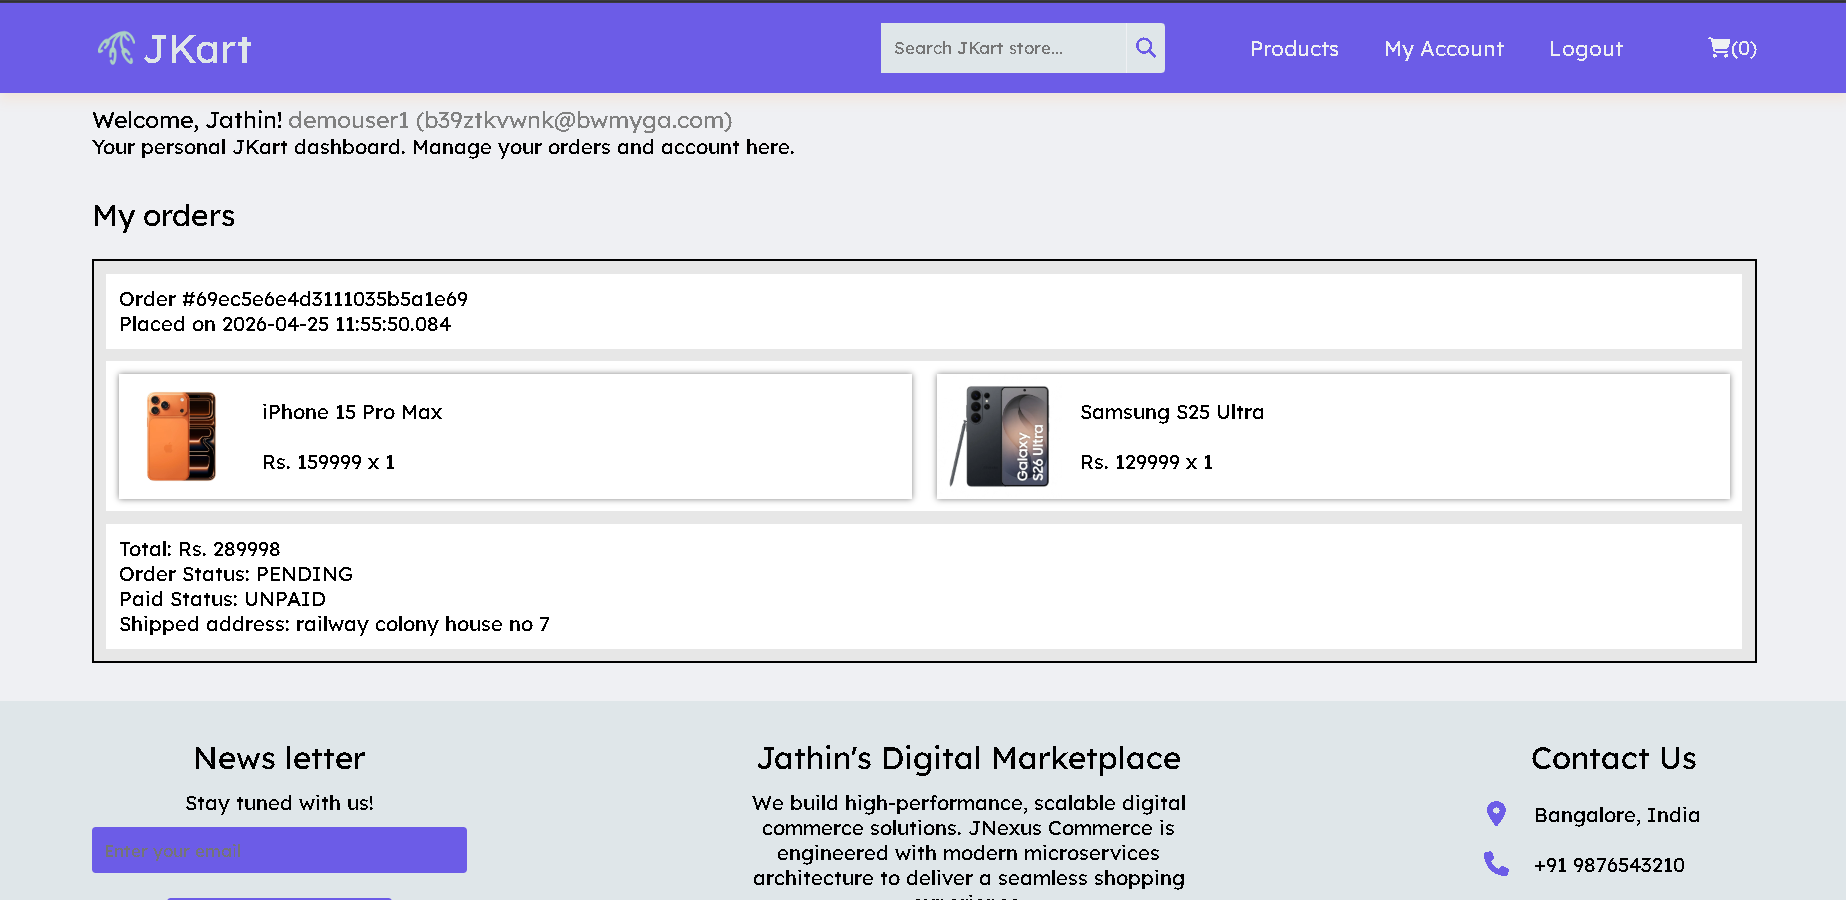
\includegraphics[width=0.85\textwidth]{orders_page.png}
\caption{User's order history page}
\label{fig:orders}
\end{figure}

Features:
\begin{itemize}
    \item List of all user's orders
    \item Each order shows: order ID, date, items, total, status
    \item Status badges: PENDING (yellow), SUCCESS (green), DELIVERED (blue)
    \item Fetches from \texttt{/api/order/get/byUser} endpoint
\end{itemize}

\section{Deployment Implementation}

\subsection{Docker Containerization}

Multi-stage Dockerfile for Java services:

\begin{verbatim}
FROM maven:3.9-eclipse-temurin-21 AS build
WORKDIR /app
COPY pom.xml .
RUN mvn dependency:go-offline
COPY src ./src
RUN mvn package -DskipTests

FROM eclipse-temurin:21-jre
WORKDIR /app
COPY --from=build /app/target/*.jar app.jar
EXPOSE 8080
ENTRYPOINT ["java", "-jar", "app.jar"]
\end{verbatim}

Benefits:
\begin{itemize}
    \item Separate build and runtime stages
    \item Final image contains only JRE (smaller size)
    \item No build tools in production image
    \item Reduced attack surface
\end{itemize}

\subsection{Kubernetes Deployment}

Each service deployed via Helm chart:

\begin{verbatim}
apiVersion: apps/v1
kind: Deployment
metadata:
  name: {{ .Values.service.name }}
spec:
  replicas: {{ .Values.replicaCount }}
  selector:
    matchLabels:
      app: {{ .Values.service.name }}
  template:
    spec:
      containers:
        - name: {{ .Values.service.name }}
          image: {{ .Values.image.repository }}:{{ .Values.image.tag }}
          ports:
            - containerPort: {{ .Values.service.port }}
          env:
            - name: SPRING_DATA_MONGODB_URI
              valueFrom:
                secretKeyRef:
                  name: mongodb-secret
                  key: uri
\end{verbatim}

\subsection{AWS Infrastructure (Terraform)}

Provisioned resources:
\begin{itemize}
    \item VPC with public and private subnets
    \item Internet Gateway and NAT Gateway
    \item EKS cluster with managed node groups
    \item ECR registries for each service
    \item ALB for ingress routing
    \item IAM roles and policies
\end{itemize}

\subsection{CI/CD Pipeline (GitHub Actions)}

Example workflow for Product Service:

\begin{verbatim}
name: Product Service CI/CD
on:
  push:
    paths:
      - 'microservice-backend/product-service/**'
jobs:
  build-and-deploy:
    runs-on: ubuntu-latest
    steps:
      - uses: actions/checkout@v3
      - name: Configure AWS credentials
        uses: aws-actions/configure-aws-credentials@v2
      - name: Login to ECR
        uses: aws-actions/amazon-ecr-login@v1
      - name: Build Docker image
        run: docker build -t product-service .
      - name: Push to ECR
        run: docker push <ecr-url>:latest
      - name: Deploy to EKS
        run: helm upgrade product-service ./helm/product-service
\end{verbatim}

\section{Testing Results}

\subsection{Unit Testing}

\begin{table}[h!]
\centering
\caption{Unit Test Coverage by Service}
\begin{tabular}{|l|c|c|}
\hline
\textbf{Service} & \textbf{Tests} & \textbf{Coverage (\%)} \\
\hline
Auth Service & 42 & 85 \\
User Service & 28 & 82 \\
Category Service & 24 & 80 \\
Product Service & 38 & 84 \\
Cart Service & 32 & 83 \\
Order Service & 35 & 81 \\
Notification Service & 18 & 78 \\
\hline
\textbf{Total} & \textbf{217} & \textbf{82} \\
\hline
\end{tabular}
\end{table}

\subsection{Integration Testing}

Tested scenarios:
\begin{itemize}
    \item User registration $\rightarrow$ OTP verification $\rightarrow$ login flow
    \item Product creation (admin) $\rightarrow$ browsing $\rightarrow$ search
    \item Add to cart with user/product validation
    \item Order placement with cart clearing
    \item Email notification delivery
\end{itemize}

All critical flows passed successfully with expected behavior.

\subsection{Performance Testing}

\begin{table}[h!]
\centering
\caption{API Response Times}
\begin{tabular}{|l|c|}
\hline
\textbf{Endpoint} & \textbf{Avg Response (ms)} \\
\hline
Product listing & 120 \\
Product search & 180 \\
Add to cart & 250 \\
Place order & 420 \\
Login & 150 \\
\hline
\end{tabular}
\end{table}

All endpoints meet performance requirements (< 500ms for most operations).

\section{Challenges and Solutions}

\subsection{Challenge 1: Inter-Service Validation}

\textbf{Problem:} Cart Service needs to validate user and product exist before adding items.\\
\textbf{Solution:} Implemented OpenFeign clients calling User Service and Product Service. Added error handling for service unavailability.\\
\textbf{Outcome:} Successful validation with graceful error messages.

\subsection{Challenge 2: JWT Token Validation Across Services}

\textbf{Problem:} Each service needs to validate tokens without duplicating logic.\\
\textbf{Solution:} Created reusable \texttt{AuthTokenFilter} in each service calling Auth Service via Feign.\\
\textbf{Outcome:} Centralized authentication with consistent security across all services.

\subsection{Challenge 3: MongoDB Database Isolation}

\textbf{Problem:} Ensuring each service uses its own database.\\
\textbf{Solution:} Configured separate \texttt{spring.data.mongodb.uri} in each service's \texttt{application.yml}.\\
\textbf{Outcome:} Proper data isolation with independent database per service.

\subsection{Challenge 4: CORS Configuration}

\textbf{Problem:} Frontend on port 5173 blocked from calling API Gateway on port 8080.\\
\textbf{Solution:} Configured CORS in API Gateway allowing \texttt{http://localhost:5173} origin.\\
\textbf{Outcome:} Successful frontend-backend communication.

\section{Summary}

This chapter presented implementation details for all JKart components including backend microservices, React frontend, Docker containerization, Kubernetes deployment, AWS infrastructure, and CI/CD automation. Screenshots demonstrated the working application with product browsing, cart management, and order placement. Testing validated functionality with 82\% average code coverage and acceptable performance. Challenges in inter-service communication, authentication, and deployment were successfully resolved.
